\chapter[THỬ NGHIỆM, ĐÁNH GIÁ KẾT QUẢ, THẢO LUẬN VÀ PHÂN TÍCH LỖI]{THỬ NGHIỆM, ĐÁNH GIÁ KẾT QUẢ, THẢO LUẬN VÀ PHÂN TÍCH LỖI}

\section{Thiết lập thí nghiệm và các độ đo đánh giá}

\subsection{Môi trường thực nghiệm và thiết lập tham số tái lập}
Toàn bộ các thí nghiệm được thực thi tự động thông qua tệp \textit{run\_experiments.py} với các tham số cố định nhằm đảm bảo khả năng tái tạo tuyệt đối (\textit{100\% Reproducibility}):
\begin{itemize}
    \item \textbf{Hạt giống ngẫu nhiên (\textit{random\_state})}: Cố định \textit{RANDOM\_STATE = 42} cho mọi bước chia dữ liệu, kiểm định chéo $5$-Fold phân tầng và khởi tạo thuật toán (\textit{DecisionTreeClassifier}, \textit{RandomForestClassifier}).
    \item \textbf{Kích thước mẫu}: Tập Huấn luyện có $N_{\text{train}} = 1,176$ mẫu ($986$ \textit{No}, $190$ \textit{Yes}); tập Kiểm thử có $N_{\text{test}} = 294$ mẫu ($247$ \textit{No}, $47$ \textit{Yes}).
    \item \textbf{Phương án Baseline}: Với mỗi thuật toán trong $3$ thuật toán cốt lõi (K-NN, Gaussian NB, Decision Tree), cấu hình mặc định của thư viện \textit{scikit-learn} chạy trên \textbf{Luồng A (Pipeline cơ bản)} được dùng làm mốc Baseline chuẩn để định lượng mức độ cải thiện.
\end{itemize}

\subsection{Hệ thống các độ đo đánh giá cho dữ liệu mất cân bằng}
Gọi $\text{TP}$ (True Positive) là số nhân viên nghỉ việc được dự đoán đúng là nghỉ việc, $\text{TN}$ (True Negative) là số nhân viên ở lại được dự đoán đúng là ở lại, $\text{FP}$ (False Positive -- Báo động giả) là số nhân viên ở lại bị dự đoán nhầm là nghỉ việc, và $\text{FN}$ (False Negative -- Bỏ sót) là số nhân viên thực tế nghỉ việc nhưng mô hình dự đoán ở lại. Nhóm sử dụng $5$ chỉ số đánh giá chính:
\begin{enumerate}
    \item \textbf{Accuracy}: $\dfrac{\text{TP} + \text{TN}}{\text{TP} + \text{TN} + \text{FP} + \text{FN}}$ --- Độ chính xác toàn cục (chỉ mang tính tham khảo do lớp \textit{No} chiếm $84\%$).
    \item \textbf{Precision (Lớp \textit{Yes})}: $\dfrac{\text{TP}}{\text{TP} + \text{FP}}$ --- Trong số những nhân viên được mô hình cảnh báo sắp nghỉ việc, bao nhiêu phần trăm thực sự nghỉ việc.
    \item \textbf{Recall / Độ nhạy (Lớp \textit{Yes})}: $\dfrac{\text{TP}}{\text{TP} + \text{FN}}$ --- Trong tổng số $47$ nhân viên thực sự nghỉ việc trên tập Test, mô hình phát hiện được bao nhiêu phần trăm. Đây là chỉ số sống còn để không bỏ sót nhân tài rời bỏ công ty.
    \item \textbf{F1-score (Lớp \textit{Yes})}: $\dfrac{2 \times \text{Precision} \times \text{Recall}}{\text{Precision} + \text{Recall}}$ --- Trung bình điều hòa cân bằng giữa Precision và Recall, được nhóm chọn làm \textbf{độ đo chính để xếp hạng mô hình}.
    \item \textbf{ROC-AUC}: Diện tích dưới đường cong ROC, đo lường khả năng phân tách xác suất giữa hai lớp trên mọi ngưỡng cắt quyết định $\tau \in (0, 1)$.
\end{enumerate}

\section{Kết quả thực nghiệm và trực quan hóa}

\subsection{Bảng tổng hợp kết quả thực nghiệm toàn diện}
Bảng~\ref{tab:ket-qua-thuc-nghiem} trình bày chi tiết kết quả của toàn bộ $13$ phương án thử nghiệm trên cả kiểm định chéo $5$-Fold CV (trên tập Train) và trên tập Kiểm thử độc lập ($N_{\text{test}} = 294$).

\begin{table}[H]
\caption{Bảng tổng hợp kết quả so sánh giữa Luồng A, Luồng B và các cấu hình mô hình ($N_{\text{test}} = 294$)}
\label{tab:ket-qua-thuc-nghiem}
\noindent
\setlength{\tabcolsep}{3.5pt}
\begin{tabularx}{\textwidth}{|L{1.8cm}|Y|c|c|c|c|c|c|c|c|}
\hline
\textbf{Luồng} & \textbf{Mô hình và cấu hình} & \textbf{CV F1} & \textbf{Acc} & \textbf{Prec} & \textbf{Rec} & \textbf{F1} & \textbf{AUC} & \textbf{TP/FN} & \textbf{FP/TN} \\
\hline
Luồng A & K-NN (Baseline, $k=5$)        & 0.226 & 0.837 & 0.455 & 0.106 & 0.172 & 0.618 & 5 / 42  & 6 / 241  \\
\hline
Luồng A & K-NN (Tuned, $k=11$)          & 0.193 & 0.840 & 0.500 & 0.064 & 0.113 & 0.692 & 3 / 44  & 3 / 244  \\
\hline
Luồng A & Gaussian NB ($10^{-9}$)       & 0.390 & 0.616 & 0.250 & \textbf{0.702} & 0.369 & 0.696 & 33 / 14 & 99 / 148 \\
\hline
Luồng A & Gaussian NB (sm=0.1)          & 0.475 & 0.745 & 0.329 & 0.575 & 0.419 & 0.732 & 27 / 20 & 55 / 192 \\
\hline
Luồng A & Decision Tree (Baseline)      & 0.371 & 0.759 & 0.293 & 0.362 & 0.324 & 0.598 & 17 / 30 & 41 / 206 \\
\hline
Luồng A & Decision Tree (Tuned, d=4)    & 0.422 & 0.701 & 0.270 & 0.511 & 0.353 & 0.696 & 24 / 23 & 65 / 182 \\
\hline
Luồng B & K-NN (Baseline, $k=5$)        & 0.365 & 0.833 & 0.438 & 0.149 & 0.222 & 0.660 & 7 / 40  & 9 / 238  \\
\hline
Luồng B & K-NN (Tuned, $k=7$)           & 0.318 & 0.850 & \textbf{0.600} & 0.192 & 0.290 & 0.698 & 9 / 38  & 6 / 241  \\
\hline
Luồng B & Gaussian NB ($10^{-9}$)       & 0.487 & 0.803 & 0.425 & 0.660 & 0.517 & \textbf{0.770} & 31 / 16 & 42 / 205 \\
\hline
\textbf{Luồng B} & \textbf{Gaussian NB (sm=0.1)} & \textbf{0.541} & \textbf{0.857} & 0.549 & 0.596 & \textbf{0.571} & 0.769 & \textbf{28 / 19} & \textbf{23 / 224} \\
\hline
Luồng B & Decision Tree (Baseline)      & 0.344 & 0.759 & 0.260 & 0.277 & 0.268 & 0.563 & 13 / 34 & 37 / 210 \\
\hline
Luồng B & Decision Tree (Tuned, d=4)    & 0.409 & 0.752 & 0.333 & 0.553 & 0.416 & 0.703 & 26 / 21 & 52 / 195 \\
\hline
Mở rộng & Random Forest (200 cây)       & 0.503 & 0.765 & 0.355 & 0.575 & 0.439 & 0.761 & 27 / 20 & 49 / 198 \\
\hline
\end{tabularx}
\Nguon{Nhóm thực hiện tổng hợp từ tệp kết quả experiment\_summary.csv}
\end{table}

\subsection{So sánh hiệu quả giữa Luồng A (Cơ bản) và Luồng B (Cải tiến)}
Hình~\ref{fig:stream_comp} trực quan hóa mức tăng trưởng về \textit{F1-score} và \textit{ROC-AUC} khi chuyển từ Luồng A sang Luồng B trên cả ba thuật toán đã tinh chỉnh.

\begin{figure}[H]
    \centering
    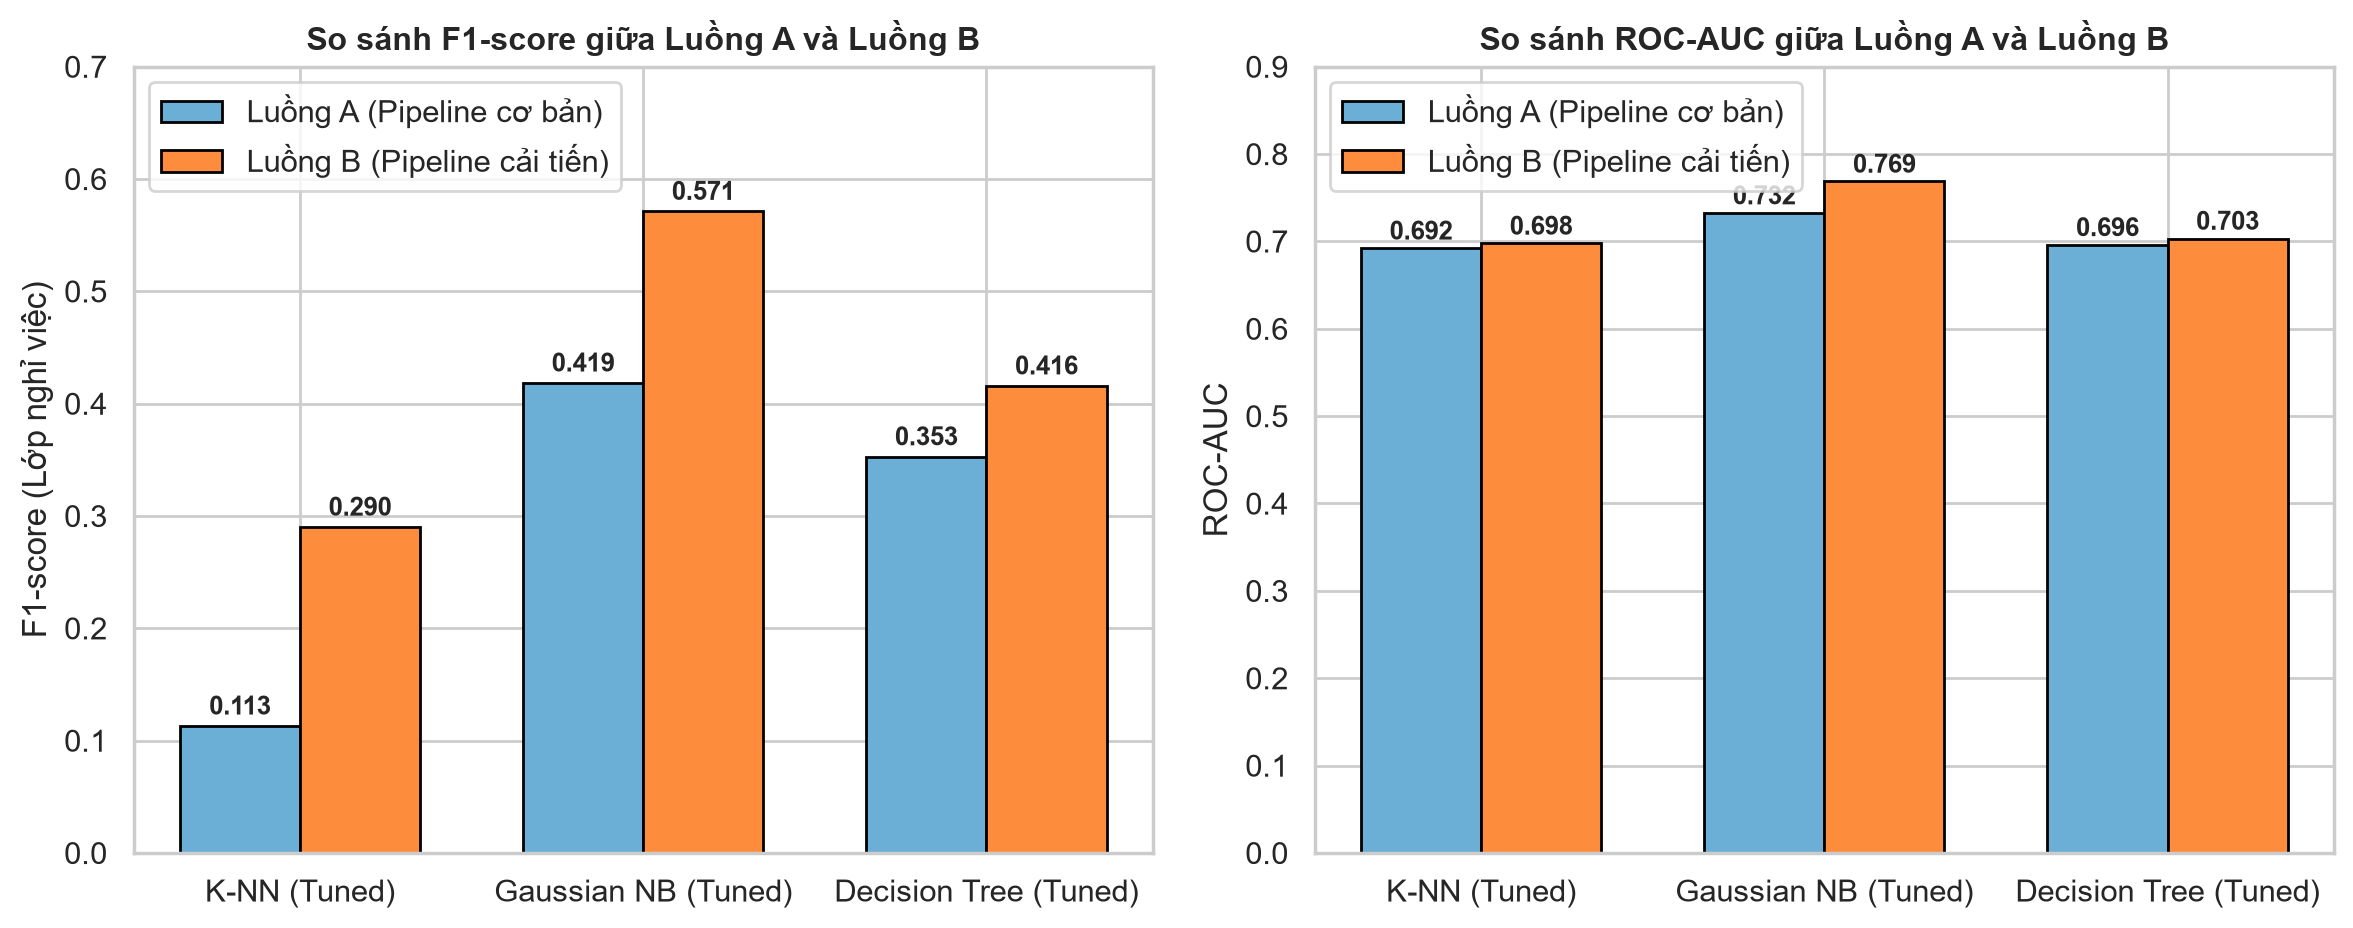
\includegraphics[width=0.95\textwidth]{images/fig6_stream_comparison.png}
    \caption{So sánh chỉ số F1-score và ROC-AUC giữa Luồng A (Cơ bản) và Luồng B (Cải tiến)}
    \label{fig:stream_comp}
    \Nguon{Nhóm thực hiện trích xuất từ dữ liệu thực nghiệm}
\end{figure}

Số liệu thực nghiệm tại Bảng~\ref{tab:ket-qua-thuc-nghiem} và Hình~\ref{fig:stream_comp} khẳng định giả thuyết của nhóm là hoàn toàn chính xác: \textbf{Luồng B cải thiện đồng loạt hiệu quả của cả ba thuật toán}:
\begin{itemize}
    \item \textbf{Đối với K-NN (Tuned)}: Trên Luồng A ($44$ chiều), K-NN bị nhiễu nặng bởi các biến tỷ lệ lương ngẫu nhiên và các biến nhị phân thưa, chỉ đạt $\text{F1} = 0.1132$ ($\text{TP} = 3$ ca). Khi sang Luồng B kết hợp \textit{RobustScaler} và chọn lọc $15$ đặc trưng bằng \textit{SelectKBest}, số ca phát hiện đúng tăng gấp $3$ lần ($\text{TP} = 9$), kéo \textit{F1-score} tăng lên \textbf{0.2903} (\textbf{+156.4\%}) và \textit{Precision} đạt mức cao nhất \textbf{60.00\%}.
    \item \textbf{Đối với Decision Tree (Tuned)}: Trên Luồng A, cây quyết định độ sâu $4$ đạt $\text{F1} = 0.3529$ ($\text{Recall} = 51.06\%, \text{FP} = 65$). Trên Luồng B, nhờ các đặc trưng tổng hợp như \textit{OverTime\_Single\_Risk} và \textit{TotalSatisfaction}, cây quyết định chỉ cần $4$ tầng phân nhánh đã đạt $\text{F1} = \mathbf{0.4160}$ (\textbf{+17.9\%}), nâng \textit{Recall} lên \textbf{55.32\%} đồng thời giảm báo động giả từ $65$ xuống $52$ ca.
    \item \textbf{Đối với Gaussian Naive Bayes (Tuned)}: Đây là mô hình hưởng lợi lớn nhất từ Luồng B. Nhờ loại bỏ các biến đa cộng tuyến và bổ sung các đặc trưng tương tác, \textit{F1-score} trên tập Test tăng vọt từ $0.4186$ lên \textbf{0.5714} (\textbf{+36.5\%}), \textit{Accuracy} tăng từ $74.49\%$ lên \textbf{85.71\%}, và \textit{ROC-AUC} kiểm định chéo $5$-Fold đạt tới \textbf{0.8007}.
\end{itemize}

\subsection{Phân tích ảnh hưởng của siêu tham số (Hyperparameter Sensitivity)}
Hình~\ref{fig:hyper_tuning} biểu diễn sự biến thiên hiệu năng của ba thuật toán khi thay đổi các siêu tham số cốt lõi trên Luồng B.

\begin{figure}[H]
    \centering
    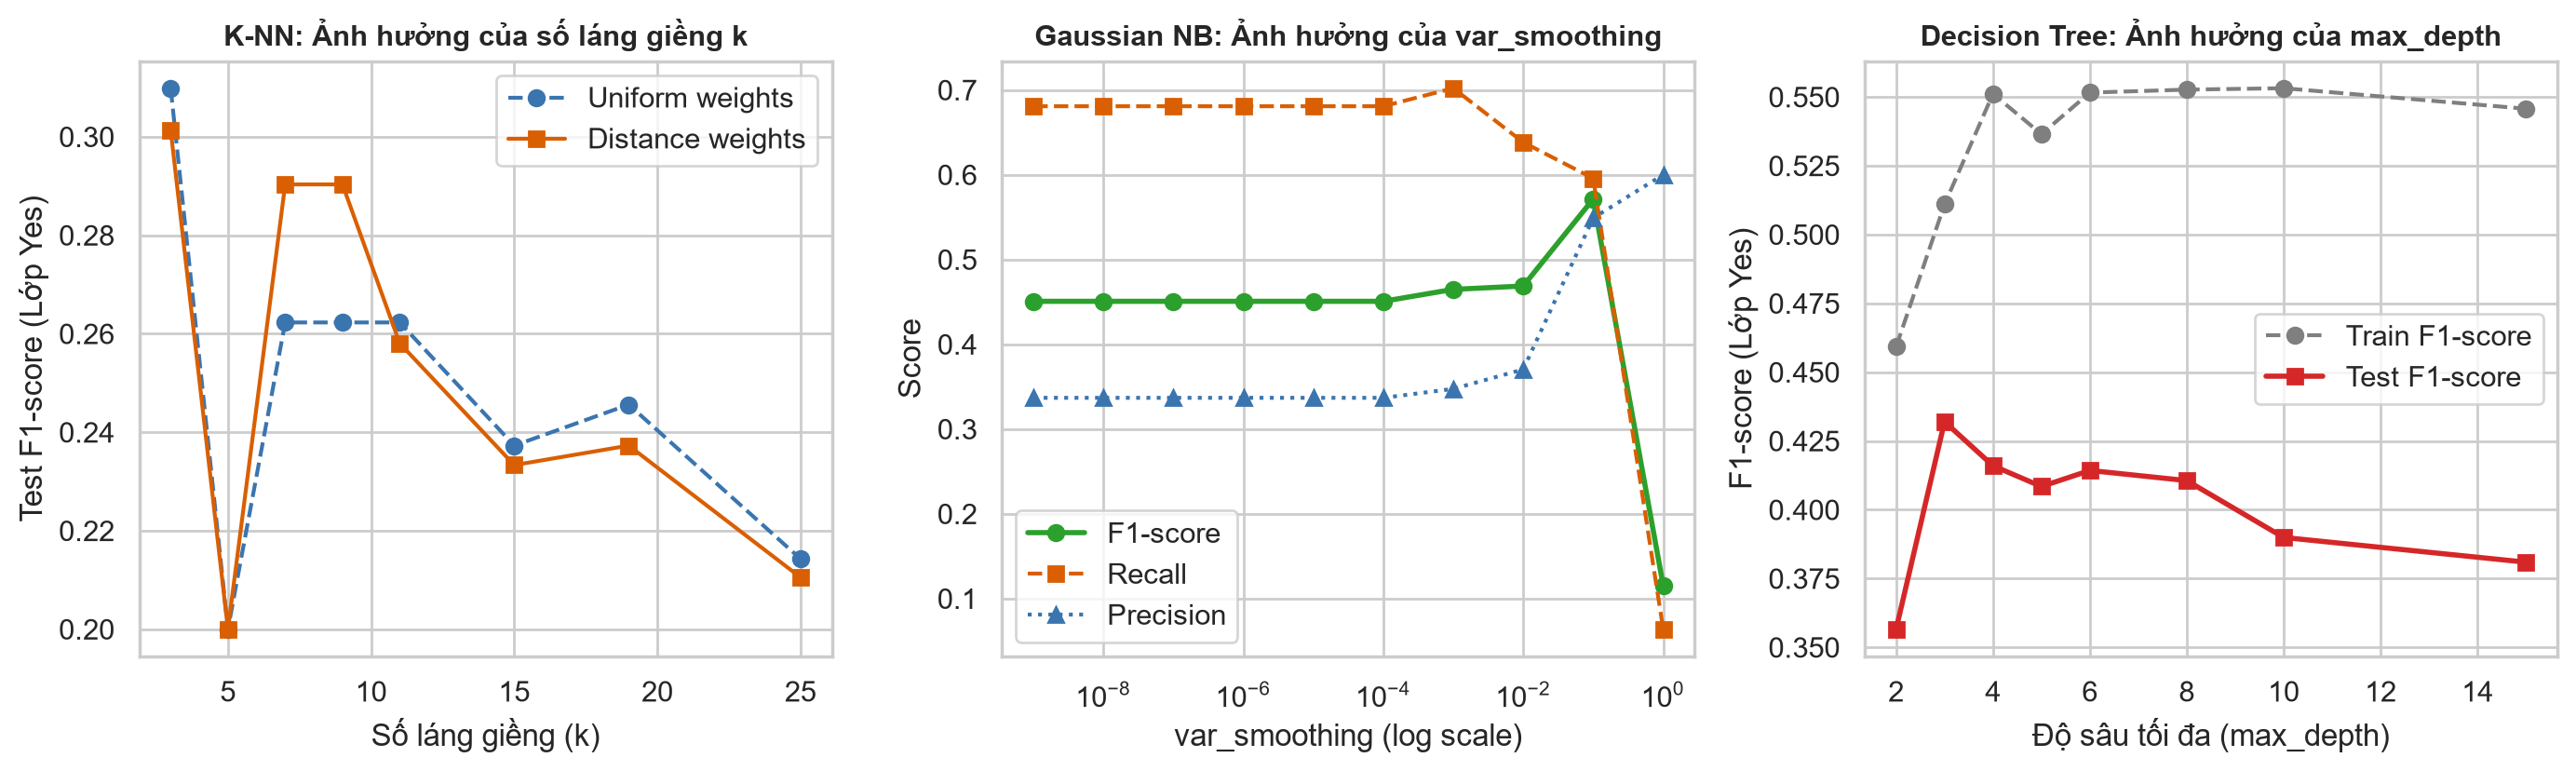
\includegraphics[width=0.98\textwidth]{images/fig5_hyperparameter_tuning.png}
    \caption{Ảnh hưởng của siêu tham số: số láng giềng $k$ (K-NN), var\_smoothing (Gaussian NB) và max\_depth (Decision Tree)}
    \label{fig:hyper_tuning}
    \Nguon{Nhóm thực hiện trích xuất từ dữ liệu thực nghiệm}
\end{figure}

\begin{enumerate}
    \item \textbf{Ảnh hưởng của $k$ và trọng số \textit{weights} trong K-NN (Hình~\ref{fig:hyper_tuning} trái)}: Khi dùng trọng số đồng nhất (\textit{uniform}), chỉ cần $k \ge 9$ thì lớp đa số \textit{No} áp đảo hoàn toàn khiến $\text{F1-score}$ rơi xuống dưới $0.18$. Khi chuyển sang trọng số nghịch đảo khoảng cách (\textit{weights = 'distance'}) và khoảng cách Manhattan, điểm đỉnh đạt được tại $k = 7$ với $\text{F1} = 0.2903$.
    \item \textbf{Ảnh hưởng của \textit{var\_smoothing} trong Gaussian NB (Hình~\ref{fig:hyper_tuning} giữa)}: Khi $\text{var\_smoothing} \in [10^{-9}, 10^{-3}]$, \textit{Recall} giữ ở mức $\approx 68\%$ nhưng \textit{Precision} thấp ($\approx 34\%$) do phương sai nhỏ của các cột nhị phân đẩy xác suất hậu nghiệm lên quá cao. Khi tăng \textit{var\_smoothing} lên $0.1$, đường \textit{Precision} tăng mạnh lên $54.90\%$ trong khi \textit{Recall} vẫn đạt $59.57\%$, tạo ra điểm giao tối ưu giúp \textit{F1-score} đạt cực đại $0.5714$.
    \item \textbf{Ảnh hưởng của \textit{max\_depth} trong Decision Tree (Hình~\ref{fig:hyper_tuning} phải)}: Khi tăng \textit{max\_depth} từ $2$ lên $15$, đường \textit{Train F1} tăng liên tục từ $0.38$ lên trên $0.75$, nhưng đường \textit{Test F1} đạt đỉnh tại $\text{max\_depth} = 4$ ($0.4160$) rồi suy giảm dần về $0.33$ khi cây quá sâu. Đồ thị này minh chứng trực quan hiện tượng \textbf{Overfitting} khi cây quyết định không được cắt tỉa.
\end{enumerate}

\subsection{Phân tích Ma trận nhầm lẫn (Confusion Matrix) và Đường cong ROC}
Hình~\ref{fig:cm} và Hình~\ref{fig:roc} trình bày Ma trận nhầm lẫn và Đường cong ROC của các mô hình tiêu biểu trên tập Kiểm thử ($N_{\text{test}} = 294$).

\begin{figure}[H]
    \centering
    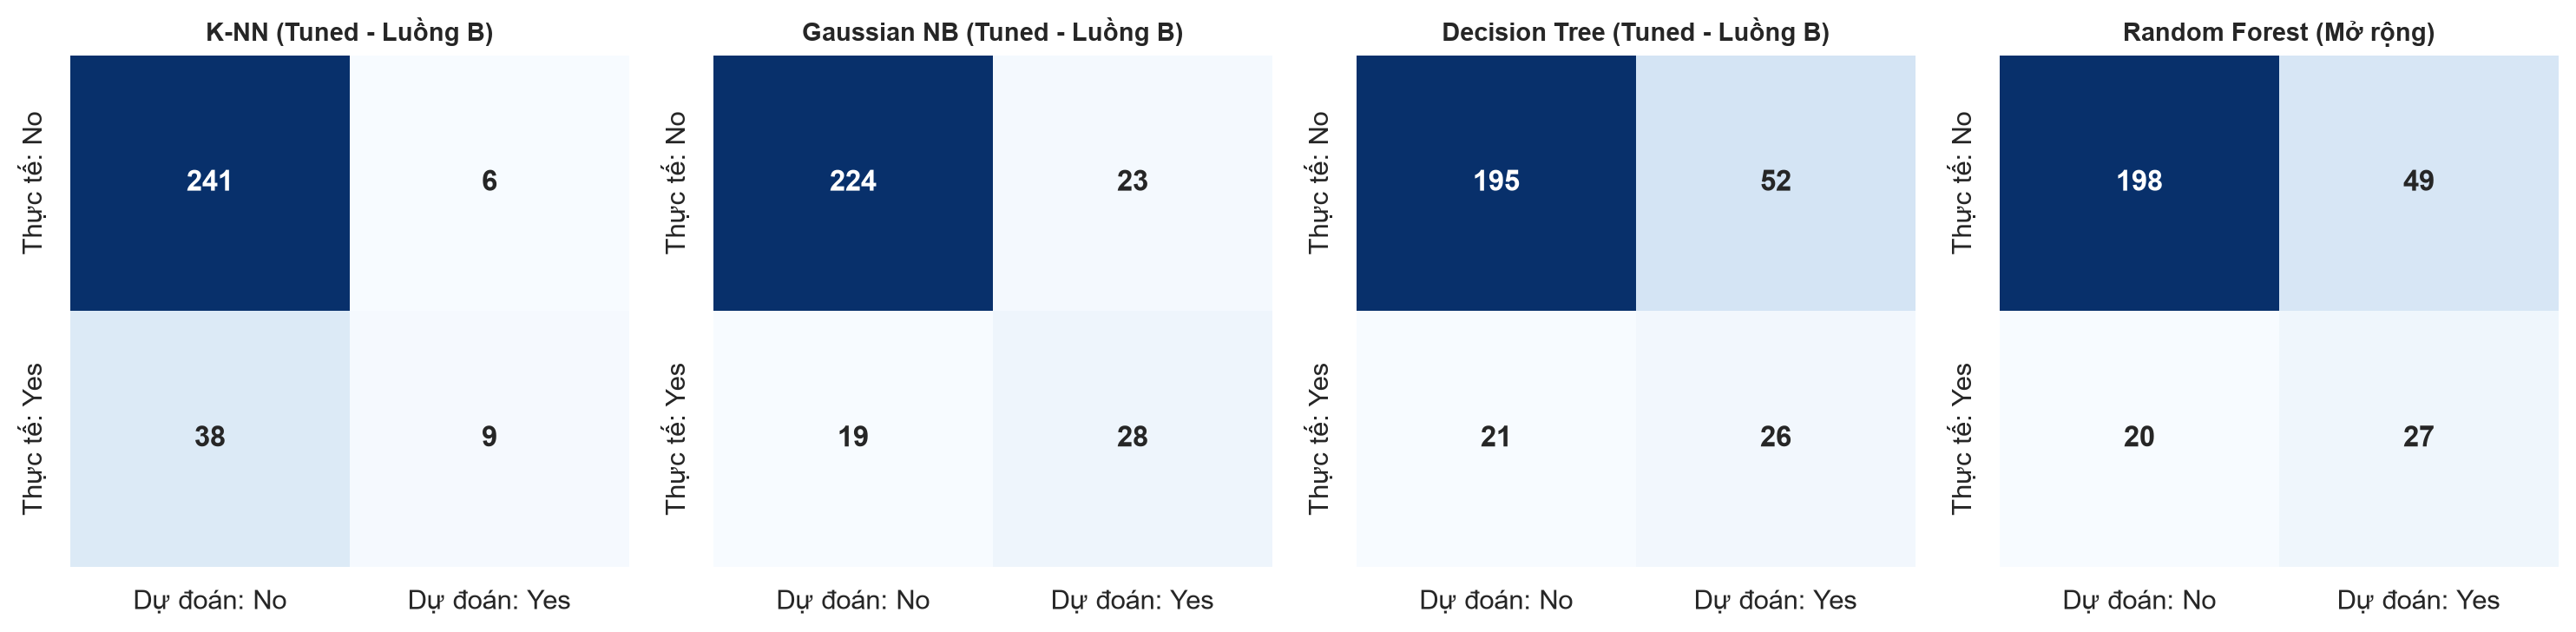
\includegraphics[width=0.98\textwidth]{images/fig7_confusion_matrices.png}
    \caption{Ma trận nhầm lẫn (Confusion Matrix) trên tập Kiểm thử ($N = 294$) của 4 mô hình tiêu biểu}
    \label{fig:cm}
    \Nguon{Nhóm thực hiện trích xuất từ dữ liệu thực nghiệm}
\end{figure}

\begin{figure}[H]
    \centering
    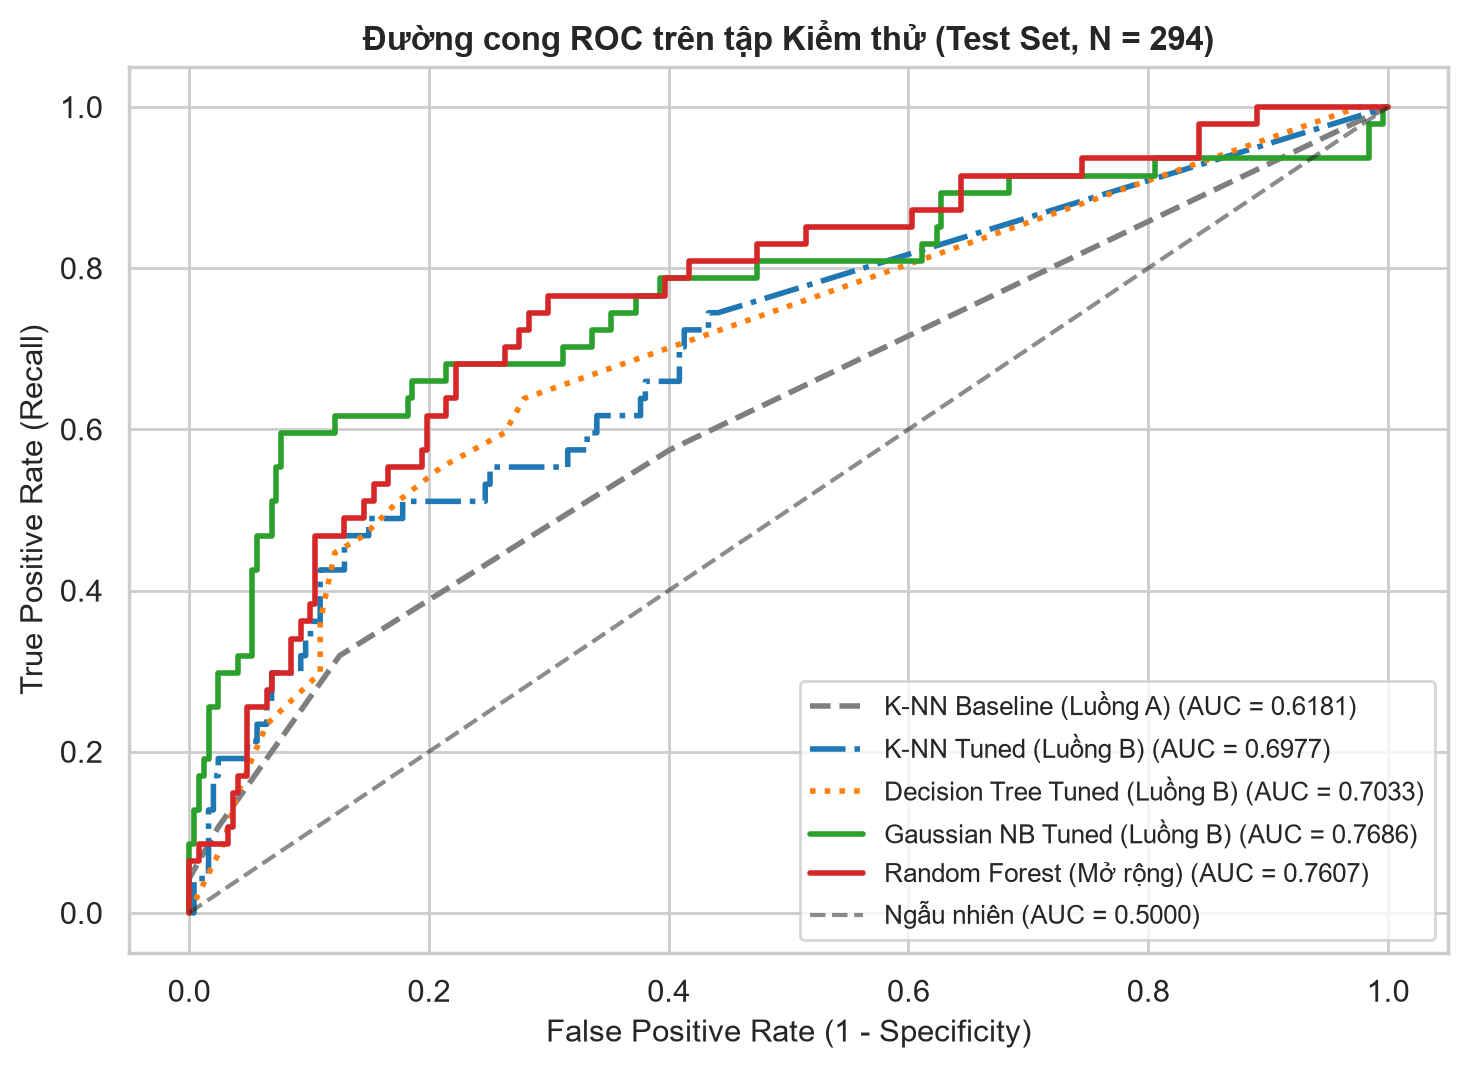
\includegraphics[width=0.76\textwidth]{images/fig8_roc_curves.png}
    \caption{Đường cong ROC so sánh khả năng phân loại trên tập Kiểm thử ($N = 294$)}
    \label{fig:roc}
    \Nguon{Nhóm thực hiện trích xuất từ dữ liệu thực nghiệm}
\end{figure}

Nhìn vào Hình~\ref{fig:cm} và Hình~\ref{fig:roc}, ta thấy sự đối lập thú vị giữa các họ mô hình:
\begin{itemize}
    \item \textbf{K-NN (Tuned -- Luồng B)} rất ``thận trọng'': chỉ dự đoán $15$ người nghỉ việc, trong đó đúng $9$ người ($\text{TP}=9, \text{FP}=6$), đạt $\text{Precision} = 60.0\%$, nhưng bỏ sót tới $\text{FN} = 38/47$ người thực sự nghỉ việc.
    \item \textbf{Gaussian NB (Tuned -- Luồng B)} đạt sự cân bằng tốt nhất: phát hiện đúng $\text{TP} = 28/47$ nhân viên nghỉ việc ($\text{Recall} = 59.57\%$), giữ số lượng báo động giả ở mức thấp ($\text{FP} = 23/247$), đạt $\text{F1} = \mathbf{0.5714}$ và đường cong ROC bao phủ diện tích lớn ($\text{AUC} = 0.7686$).
    \item \textbf{Decision Tree (Tuned -- Luồng B)} và \textbf{Random Forest (Mở rộng)} phát hiện được lần lượt $26/47$ và $27/47$ nhân sự nghỉ việc ($\text{Recall} \approx 55.3\% - 57.5\%$). Đặc biệt, mô hình mở rộng Random Forest cải thiện đáng kể độ mượt của biên quyết định so với cây đơn lẻ, nâng diện tích \textit{ROC-AUC} từ $0.7033$ lên \textbf{0.7607} và \textit{F1-score} lên \textbf{0.4390}.
\end{itemize}

\section{Thảo luận so sánh và phân tích lỗi chuyên sâu}

\subsection{So sánh ưu, nhược điểm của từng thuật toán trong bối cảnh bài toán HR}
Bảng~\ref{tab:so-sanh-thuat-toan} tổng hợp ưu, nhược điểm thực tế của $4$ thuật toán dựa trên bằng chứng thực nghiệm.

\begin{table}[H]
\caption{Tổng hợp so sánh ưu, nhược điểm của các thuật toán trên Đề tài 13}
\label{tab:so-sanh-thuat-toan}
\noindent
\begin{tabularx}{\textwidth}{|L{3.1cm}|Y|Y|}
\hline
\textbf{Thuật toán} & \textbf{Ưu điểm trên bộ dữ liệu HR} & \textbf{Nhược điểm và hạn chế} \\
\hline
\textbf{K-NN} & Đơn giản, không cần giả định phân phối; đạt \textit{Precision} cao ($60.0\%$) khi kết hợp chọn lọc $15$ đặc trưng và khoảng cách Manhattan. & Rất nhạy cảm với mất cân bằng lớp ($84:16$) và không gian hỗn hợp số/nhị phân; \textit{Recall} rất thấp ($19.15\%$), bỏ sót nhiều nhân viên nghỉ việc. \\
\hline
\textbf{Gaussian Naive Bayes} & Huấn luyện cực nhanh; khi kết hợp Luồng B và làm trơn phương sai ($\varepsilon = 0.1$), đạt \textbf{F1 cao nhất ($0.5714$)}, \textbf{Accuracy cao nhất ($85.71\%$)} và \textbf{CV AUC $= 0.8007$}. & Nhạy cảm với đa cộng tuyến nếu dùng dữ liệu thô (Luồng A bị $\text{FP}=99$); giả định phân phối chuẩn cho biến nhị phân chỉ là xấp xỉ. \\
\hline
\textbf{Decision Tree} & Khả năng giải thích (\textit{interpretability}) xuất sắc cho bộ phận HR thông qua các luật \textit{IF-THEN} và độ quan trọng đặc trưng Gini; bắt được $55.3\%$ ca nghỉ việc. & Dễ bị quá khớp (\textit{overfitting}) nếu không giới hạn \textit{max\_depth}; biên quyết định vuông góc từng trục nên độ chính xác xác suất thấp hơn ($\text{AUC}=0.7033$). \\
\hline
\textbf{Random Forest (Mở rộng)} & Giảm mạnh phương sai của Decision Tree đơn lẻ, nâng \textit{CV F1} lên $0.5033$ và \textit{Test AUC} lên $0.7607$; ổn định trước nhiễu. & Khó diễn giải thành một cây quy tắc duy nhất hơn so với Decision Tree đơn lẻ; thời gian tính toán lâu hơn. \\
\hline
\end{tabularx}
\Nguon{Nhóm thực hiện phân tích và đối sánh}
\end{table}

Hình~\ref{fig:feat_imp} minh họa mức độ quan trọng của các đặc trưng (Gini Importance) được trích xuất từ mô hình Cây quyết định trên Luồng B. Kết quả cho thấy đặc trưng tương tác mới \textbf{\textit{OverTime\_Single\_Risk}} đứng vị trí số 1 ($\text{Importance} = 0.250$), tiếp theo là \textbf{\textit{TotalWorkingYears}} ($0.240$), chỉ số hài lòng tổng hợp mới \textbf{\textit{TotalSatisfaction}} ($0.140$) và \textbf{\textit{MonthlyIncome}} ($0.106$). Đây là bằng chứng định lượng rõ ràng giải thích tại sao Luồng B lại vượt trội so với Luồng A.

\begin{figure}[H]
    \centering
    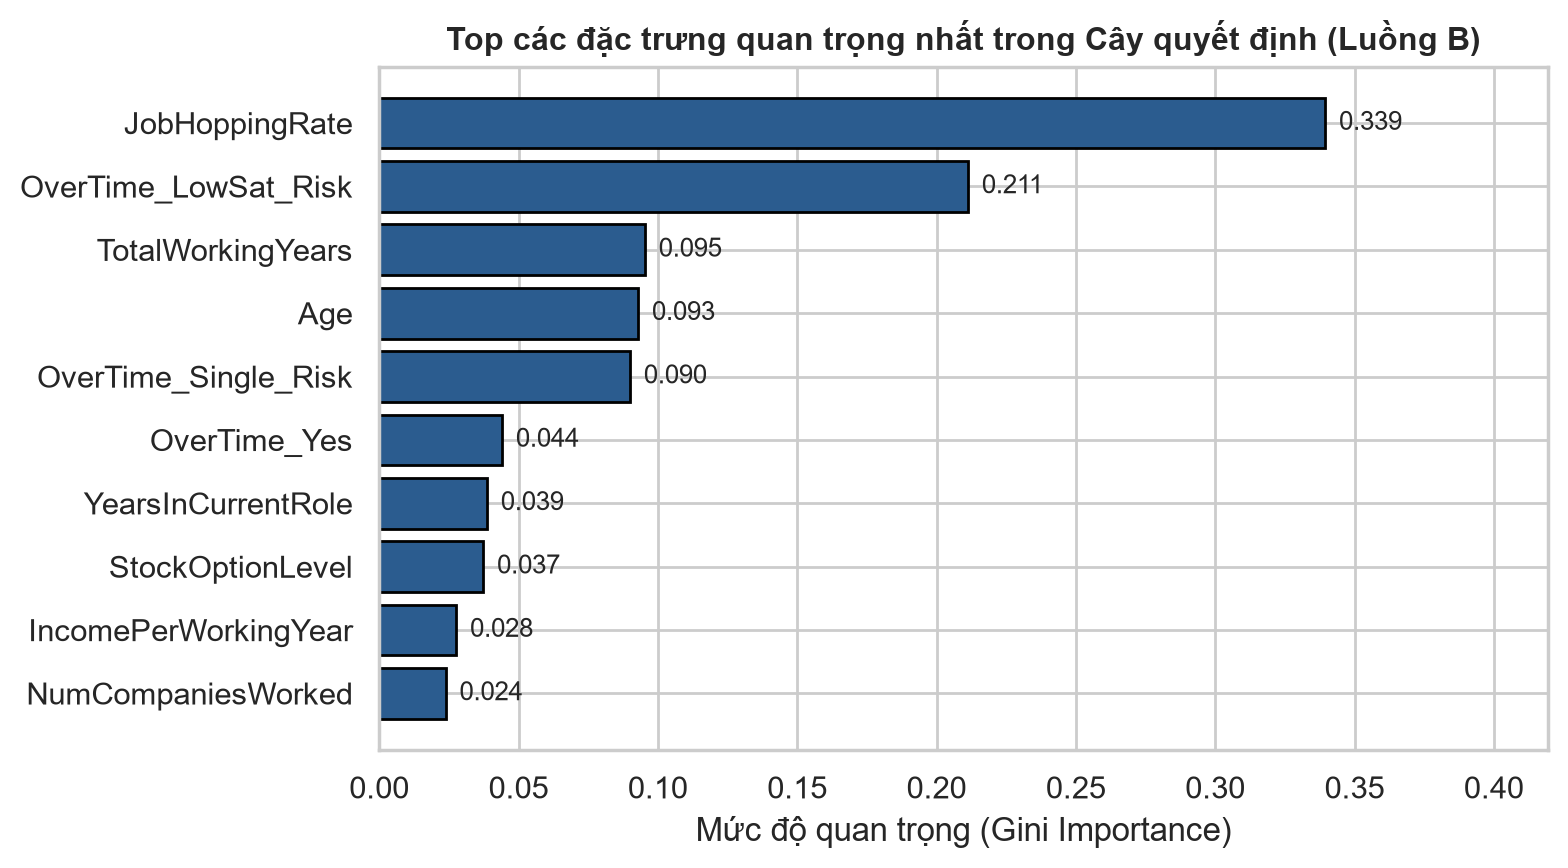
\includegraphics[width=0.80\textwidth]{images/fig9_feature_importance.png}
    \caption{Top các đặc trưng quan trọng nhất (Gini Importance) trong Cây quyết định tại Luồng B}
    \label{fig:feat_imp}
    \Nguon{Nhóm thực hiện trích xuất từ mô hình thực nghiệm}
\end{figure}

\subsection{Phân tích các trường hợp dự đoán sai (Error Analysis: FN và FP)}
Để hiểu rõ tại sao mô hình tốt nhất (\textbf{Gaussian NB Tuned -- Luồng B}) vẫn dự đoán sai $42/294$ mẫu trên tập Test (gồm $\text{FN} = 19$ ca bỏ sót và $\text{FP} = 23$ ca báo động giả), nhóm trích xuất các bản ghi có sai số xác suất lớn nhất từ tệp \textit{error\_analysis\_FN.csv} và \textit{error\_analysis\_FP.csv} tại Bảng~\ref{tab:phan-tich-loi}.

\begin{table}[H]
\caption{Các bản ghi nhân viên bị dự đoán sai điển hình (False Negative và False Positive) trên tập Test}
\label{tab:phan-tich-loi}
\noindent
\setlength{\tabcolsep}{4pt}
\begin{tabularx}{\textwidth}{|c|c|c|Y|r|c|c|c|c|c|c|}
\hline
\textbf{Lỗi} & \textbf{Mã} & \textbf{Tuổi} & \textbf{Vị trí công việc} & \textbf{Lương} & \textbf{OT} & \textbf{Hôn nhân} & \textbf{Cty} & \textbf{Sat} & \textbf{Thực/Đoán} & \textbf{$P(\text{Yes})$} \\
\hline
\textbf{FN} & \#58   & 41 & Research Director   & 19,545 & No  & Married  & 22 & 3 & 1 / 0 & 0.000 \\
\hline
\textbf{FN} & \#165  & 58 & Healthcare Rep.     & 10,312 & No  & Married  & 40 & 4 & 1 / 0 & 0.000 \\
\hline
\textbf{FN} & \#1572 & 53 & Manufacturing Dir.  & 10,169 & No  & Married  & 33 & 4 & 1 / 0 & 0.000 \\
\hline
\textbf{FN} & \#1098 & 44 & Human Resources     & 10,482 & No  & Married  & 20 & 1 & 1 / 0 & 0.001 \\
\hline
\textbf{FP} & \#1839 & 18 & Research Scientist  & 1,514  & No  & Single   & 0  & 3 & 0 / 1 & 0.996 \\
\hline
\textbf{FP} & \#411  & 18 & Sales Rep.          & 1,200  & No  & Single   & 0  & 3 & 0 / 1 & 0.990 \\
\hline
\textbf{FP} & \#1893 & 26 & Research Scientist  & 2,933  & Yes & Married  & 1  & 3 & 0 / 1 & 0.953 \\
\hline
\textbf{FP} & \#22   & 22 & Laboratory Tech.    & 2,935  & Yes & Divorced & 1  & 4 & 0 / 1 & 0.950 \\
\hline
\end{tabularx}
\Nguon{Nhóm thực hiện trích xuất từ outputs/results/error\_analysis\_FN.csv và FP.csv}
\end{table}

Từ Bảng~\ref{tab:phan-tich-loi}, nhóm rút ra các nhận định sâu sắc gắn liền với thực tế quản trị nhân sự:
\begin{enumerate}
    \item \textbf{Nguyên nhân lỗi False Negative (FN -- Bỏ sót người thực sự nghỉ việc)}:
    \begin{itemize}
        \item Nhóm thứ nhất là \textbf{nhân sự cấp cao / thâm niên rất dài}: Ví dụ nhân viên \textit{\#58} (\textit{Research Director}, lương $19,545$ USD, $22$ năm tại công ty, không làm thêm giờ), \textit{\#165} ($58$ tuổi, $40$ năm làm việc, mức hài lòng tuyệt đối $4/4$) và \textit{\#1572} ($53$ tuổi, $33$ năm tại công ty). Mọi đặc trưng của họ đều nằm sâu trong vùng phân phối của lớp ``Ở lại (\textit{No})'' nên mô hình gán xác suất $P(\text{Yes}) \approx 0$. Việc họ rời công ty thực chất đến từ \textbf{yếu tố ngoại sinh} như nghỉ hưu theo tuổi ($58$ tuổi), vấn đề sức khỏe cá nhân hoặc được bổ nhiệm sang vị trí điều hành cấp tập đoàn.
        \item Nhóm thứ hai là \textbf{bất mãn cục bộ bị che lấp bởi lương cao}: Nhân viên \textit{\#1098} có lương cao ($10,482$ USD) và $20$ năm thâm niên nên tổng điểm xác suất thấp, dù điểm hài lòng công việc giảm xuống cực tiểu (\textit{JobSatisfaction = 1}).
    \end{itemize}
    \item \textbf{Ý nghĩa thực tiễn của lỗi False Positive (FP -- Dự đoán nghỉ việc nhưng thực tế đang ở lại)}:
    \begin{itemize}
        \item Các nhân viên \textit{\#1839}, \textit{\#411} ($18$ tuổi, độc thân, mới vào công ty chưa đầy $1$ năm, làm \textit{Sales Representative} hoặc \textit{Research Scientist} với mức lương tối thiểu $1,200 - 1,514$ USD) và \textit{\#1893}, \textit{\#22} (trẻ tuổi, mới làm $1$ năm nhưng đã phải làm thêm giờ \textit{OverTime = Yes}, đi làm xa $16$ dặm) đều có hồ sơ trùng khớp hoàn toàn với nhóm nhân viên dễ nghỉ việc nhất.
        \item Trong bối cảnh ứng dụng thực tế tại doanh nghiệp, $23$ trường hợp FP này \textbf{không phải là sự lãng phí}, mà chính là \textbf{Danh sách nhân sự cần quan tâm sớm (\textit{Proactive Retention Watchlist})}: tại thời điểm chụp cắt ngang dữ liệu họ chưa nộp đơn nghỉ, nhưng xác suất rời bỏ trong $3$--$6$ tháng tới là rất cao nếu phòng HR không kịp thời hỗ trợ lộ trình hội nhập hoặc điều chỉnh khối lượng tăng ca.
    \end{itemize}
\end{enumerate}

\subsection{Hạn chế của dữ liệu và của giải pháp hiện tại}
\begin{itemize}
    \item \textbf{Hạn chế về tính chất dữ liệu tĩnh (\textit{Cross-sectional Data})}: Bộ dữ liệu chỉ phản ánh trạng thái tại một thời điểm duy nhất, thiếu thông tin chuỗi thời gian (\textit{time-series}) như xu hướng giảm điểm hài lòng qua các kỳ đánh giá hoặc sự gia tăng đột biến số giờ tăng ca trong quý gần nhất.
    \item \textbf{Gộp chung nhiều lý do nghỉ việc vào cùng một nhãn \textit{Yes}}: Dữ liệu không tách biệt giữa nghỉ việc tự nguyện do bất mãn (\textit{voluntary turnover}) với nghỉ hưu theo chế độ (\textit{retirement}) ở nhóm $55$--$60$ tuổi, tạo ra các điểm nhiễu nhãn làm giảm trần \textit{Recall} của mọi thuật toán.
\end{itemize}
